%type de document
\documentclass[a4paper,12pt]{article}

% regles typographiques françaises
%\usepackage[latin1]{inputenc}
\usepackage[utf8]{inputenc}
\usepackage[francais]{babel}
\usepackage[T1]{fontenc}


% mise en page
\usepackage[margin=2cm]{geometry}
\usepackage{fancyhdr}
\usepackage{graphicx}
\usepackage{array}
%\usepackage{lastpage}
%\usepackage{placeins}
%\usepackage{longtable}
%\usepackage{caption}
\usepackage{float}
\usepackage{wrapfig}
\usepackage{dirtree}

\usepackage[smaller, footnote, printonlyused]{acronym} % table d'acronymes, option [footnote] pour avoir les définitions en bas de page [printonlyused

\usepackage{hyperref}
\hypersetup{colorlinks=true, linkcolor=blue}
\hypersetup{pdfauthor=Sebastien Chassot}
\hypersetup{pdfstartpage=1}
\hypersetup{pdfpagemode=None} %FullScreen, None
\hypersetup{pdfpagelayout=SinglePage} %SinglePage, OneColumn, TwoColumnLeft, TwoColumnRight
\hypersetup{pdfstartview=FitH} %Fit, FitH, FitV, FitB, FitBH, FitBV
\pdfcompresslevel=9
%\hypersetup{
%  bookmarks=true                % show bookmarks bar?
%, bookmarksopen=true
%, unicode=false                 % non-Latin characters in Acrobat bookmarks
%, pdftoolbar=true               % show Acrobat toolbar?
%, pdfmenubar=true               % show Acrobat menu?
%, pdffitwindow=false            % window fit to page when opened
%, pdfpagemode=UseOutlines       % FullScreen, UseThumbs(show thumbnails)
%                                % UseOutlines(show bookmarks), None
%, pdfpagelayout=SinglePage      % SinglePage, OneColumn, TwoColumnLeft, TwoColumnRight
%, pdfstartpage=1
%, pdfstartview={FitV}           % Fit, FitH, FitV, FitB, FitBH, FitBV
%, pdfsubject={}
%, pdftitle={Rapport}    		% title
%, pdfauthor={J. Mendes, S. Chassot, D. Wittwer}       	% author
%, pdfcreator={LaTeX}            % creator of the document
%, pdfkeywords={HEPIA} {Rapport} {analyse} {programmation} {terminal} {c}  % list of keywords
%, pdfnewwindow=true             % links in new window
%, colorlinks=false              % false: boxed links; true: colored links
%, linkcolor=red                 % color of internal links
%, citecolor=black               % color of links to bibliography
%, filecolor=magenta             % color of file links
%  urlcolor=blue                 % color of external links
%}

% Espacement interligne
\usepackage{setspace}
\onehalfspacing

% Couleur
\usepackage{colortbl}
\definecolor{bleuClair}{rgb}{0.31,0.51,0.74}

% ligne vide
\newcommand{\emptyLine}[1][1]{\par\leavevmode\par}

% lstlisting configuration
\usepackage{fancyvrb}
\usepackage{xcolor}
\usepackage{listings}

% D�finition des couleurs
\definecolor{lightgreen}{rgb}{0.2,.98,0.2}
\definecolor{darkgreen}{rgb}{0,0.4,0}
\definecolor{lightgray}{gray}{0.98}
\definecolor{darkred}{rgb}{0.545,0.000,0.000}
\definecolor{bleuClair}{rgb}{0.31,0.51,0.74}
\definecolor{grisTableau}{rgb}{0.9529,0.9529,0.9529}
\lstset {	
  language=C
, frame=single
, keepspaces=true
, columns=fullflexible
, captionpos=b
, stepnumber=10
, morekeywords={var,get,set}
, basicstyle=\ttfamily\scriptsize
, keywordstyle=\color{blue}
, commentstyle=\color{darkgreen}
, stringstyle=\color{darkred}
, backgroundcolor=\color{white}
, numbers=left
, numberstyle=\scriptsize
, numbersep=5pt
, breaklines=true
, tabsize=3
, showstringspaces=false
, emph={double,bool,int,unsigned,char,true,false,void,get,set}
, emphstyle=\color{blue}
, emph={Assert,Test}
, emphstyle=\color{red}
, emph={[2]\#using,\#define,\#ifdef,\#endif}
, emphstyle={[2]\color{blue}}
, rulesepcolor=\color{gray}
, lineskip={-1.5pt} % single line spacing
, escapeinside={/*(*@}{@*)*/}
, rangeprefix=\{\  % curly left brace plus space
, rangesuffix=\ \} % space plus curly right brace
}
\lstset{prebreak=\raisebox{0ex}[0ex][0ex]
        {\ensuremath{\hookleftarrow}}}
%\lstset{postbreak=\raisebox{0ex}[0ex][0ex]
%        {\ensuremath{\hookrightarrow\space}}}
\lstset{breaklines=true, breakatwhitespace=true}

% replace sequence of char by another sequence of char
% see http://stackoverflow.com/questions/1116266/listings-in-latex-with-utf-8-or-at-least-german-umlauts
\lstset{literate=%
{ä}{{\"a}}1
{â}{{\^a}}1
{� }{{\`a}}1
{ë}{{\"e}}1
{ê}{{\^e}}1
{é}{{\'e}}1
{è}{{\`e}}1
{ï}{{\"i}}1
{î}{{\^i}}1
{ö}{{\"o}}1
{ô}{{\^o}}1
{ü}{{\"u}}1
{û}{{\^u}}1
{ç}{{\c c}}1
{°}{{\textsuperscript{o}}}1
% suppress BOM (Byte Order Mark) characters at the beginning of Visual Studio source
% see http://tex.stackexchange.com/questions/5935/how-to-suppress-bom-effect-in-the-output
{�}{}0
{�}{}0
{�}{}0
}

%%%%%%%%%%%%%%%%%%%%%%%%%%%%%%%%%%%%%%%%%%%%%%%%%%%%%%%%%%%%%%%%%
%		DEBUT DU DOCUMENT
%%%%%%%%%%%%%%%%%%%%%%%%%%%%%%%%%%%%%%%%%%%%%%%%%%%%%%%%%%%%%%%%%

\begin{document}

%%%%%%%%%%%%%%%%%%%%%%%%%%%%%%%%%%%%%%%%%%%%%%%%%%%%%%%%%%%%%%%%%%%
%		ENTETE ET PIED DE PAGE
%%%%%%%%%%%%%%%%%%%%%%%%%%%%%%%%%%%%%%%%%%%%%%%%%%%%%%%%%%%%%%%%%
\pagestyle{fancy}
% entête
\lhead{}
\chead{}
\rhead{}
% pied de page
\lfoot{}
\cfoot{Page \thepage\ sur \pageref{LastPage} }
\rfoot{}
\renewcommand{\headrulewidth}{0.1pt}
\renewcommand{\footrulewidth}{0.1pt}
\fancyhead[R]{\textsl{ prog system - TP Minix File system }}
%\fancyfoot[C]{\scriptsize\emph{\class}}

\fancyfoot[L]{\scriptsize\emph{\docschool{}}}


%%%%%%%%%%%%%%%%%%%%%%%%%%%%%%%%%%%%%%%%%%%%%%%%%%%%%%%%%%%%%%%%%%%

\author{Sebastien Chassot}
\newcommand{\docschool}{hepia - ITI}
\title{Rapport}

% page de titre
\begin{center}
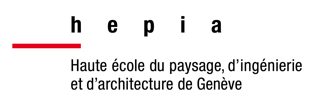
\includegraphics[scale=2]{imgs/hepia}
\end{center}

\vspace{3cm}

\begin{center}
\begin{huge}
\textbf{Rapport}
\end{huge}
\end{center}

\begin{center}
\begin{large}
Minix File system
\end{large}
\end{center}

% Trait de separation
\newcommand{\lineunder}{\color{bleuClair}\hrulefill\\\color{black}}
\lineunder

\begin{center}
\begin{large}
ITI 2\up{ème} soir \\
2014 / 2015
\end{large}
\end{center}

\vspace{3cm}
\centerline{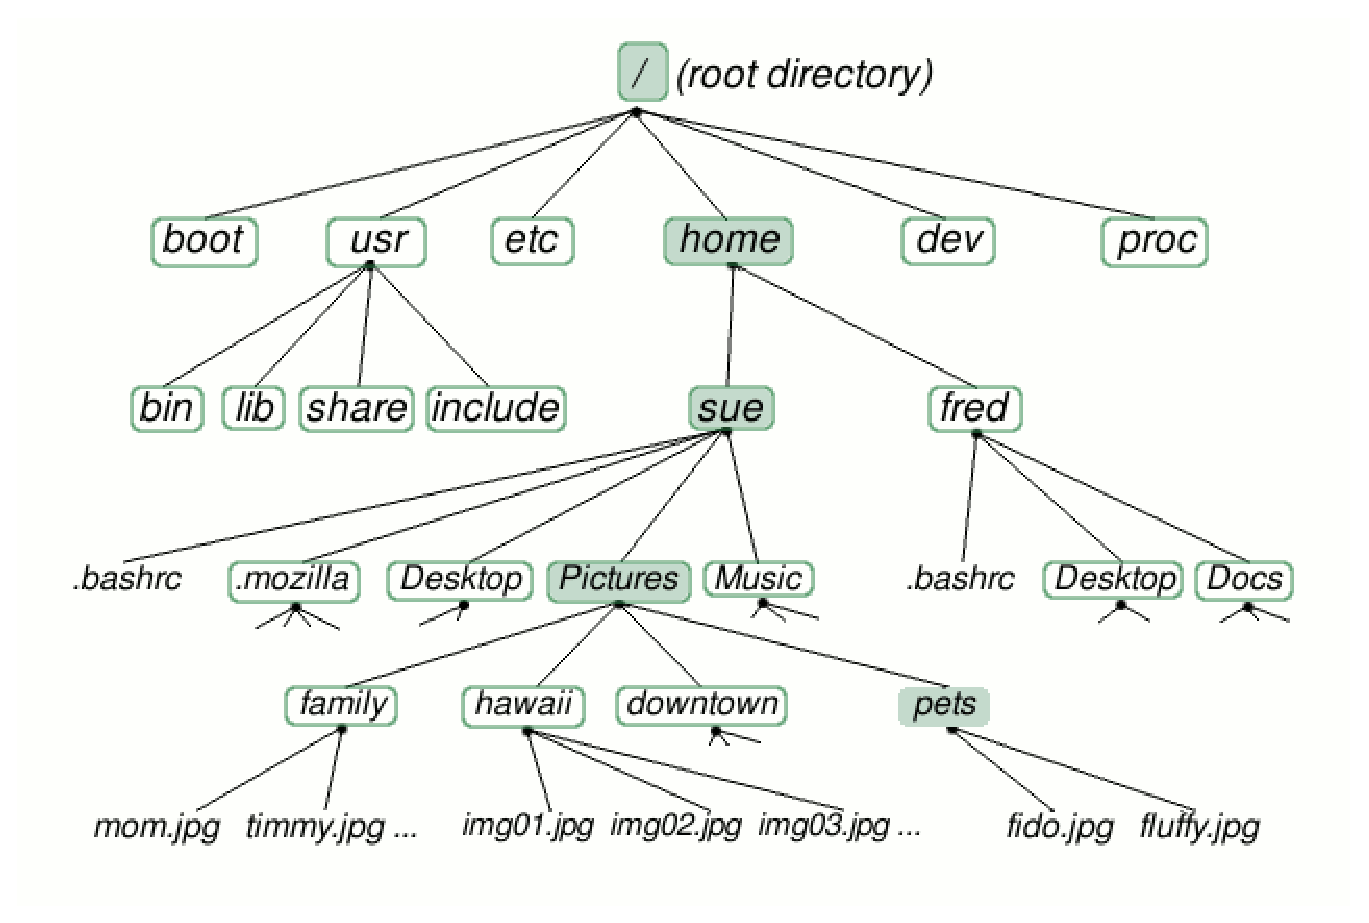
\includegraphics[scale=0.52]{imgs/illustration_FS}}
\vspace{2cm}

\begin{center}
%\begin{large}
\textbf{Sebastien Chassot} \\ Juin 2015
%\end{large}
\end{center}

\thispagestyle{empty} % enleve les entetes et pide de page de la page de titre

% table des matières
\newpage % nouvelle page
\tableofcontents % table des matières
\listoffigures
\listoftables
\newpage % nouvelle page

%\chapter*{Mini Bash}


\section{Introduction}

Le but de ce travail est d'implémenter un système MinixFS V1 en python en proposant une API standard et de modifier un fichier \emph{formaté} en minixfs via cet interface.\\

Dans un deuxième temps, les modifications seront faites à travers le réseau. Un programme de test simple écrit en python utilise l'API mais les lectures/écritures sont faite par un server de blocs. Le server (écrit en C) modifiera le fichier selon les commandes reçues au travers d'une sockets AF\_INET. On réutilisera le travail fait en python et son API mais les block seront transmis au server selon un protocole relativement simple.
 
\begin{figure}[H]
\begin{center}
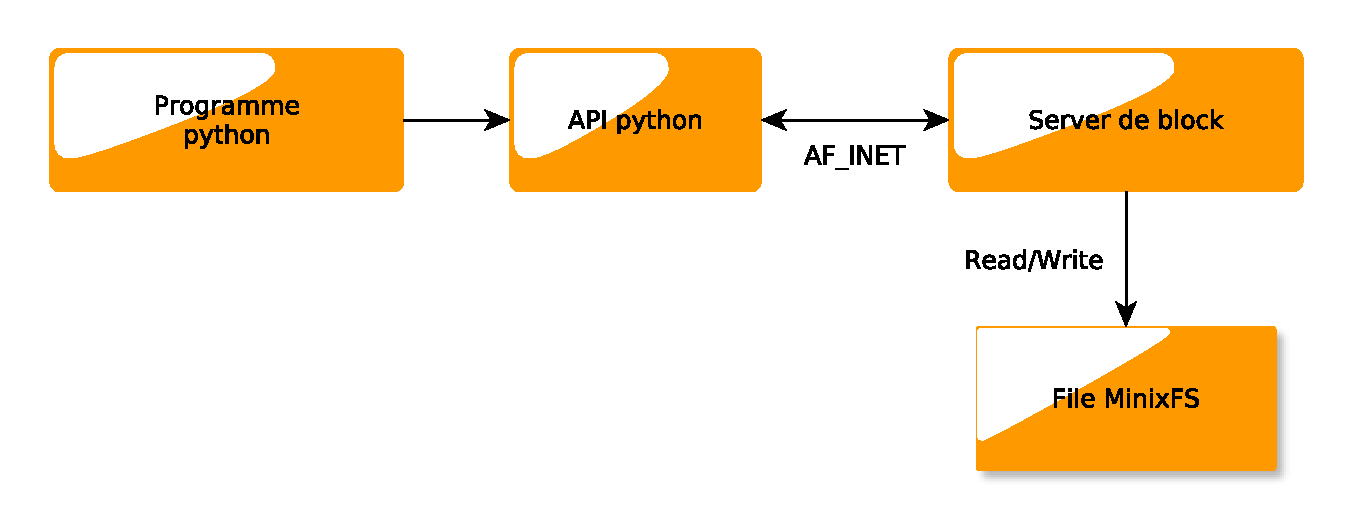
\includegraphics[scale=.6]{imgs/schema_client_server}
\caption{Principe de fonctionnement}
\label{fig:Architecture client server}
\end{center}
\end{figure}


Un seul client est traité à la fois ce qui évite les problèmes d'accès concurrent - traité dans d'autres cours. Le principe est simple; le client fait une requête, le server y répond.\\


\subsection{Exécution du programme}

Fonctionnement du programme. Toutes les commandes peuvent être lancées avec make.\\

\begin{lstlisting}[language=bash,caption={lancer le server}]

pour les tests en local

	$ make test1
ou
	$ make test2
	
pour lancer la doc
	$ make doc

	$ ./server
	Usage : ./server <port> <file>
	
	
pour lancer le server avec make
	$ make server && make run
ou avec strace
	$ make server && make run_debug
	
dans un autre terminal
	$ make test_server

\end{lstlisting}


\section{Implémentation python}

L'API implémentée est une version simplifiée d'un système de fichiers actuelle. On y retrouve les même méthodes et le fonctionnement global est le même.\\

\subsection{description de l'API}


\begin{description}
\item[ialloc()] \hfill \\
	alloue le premier inode de libre - puisqu'il contient peut-être d'ancienne donnée, il est remplacé par un nouvel inode vierge.
\item[ifree(inodenum)] \hfill \\
	change l'état de l'inode à \emph{libre} dans la bitmap des inodes. Cet inode sera donc libre pour une nouvelle allocation.
\item[balloc()] \hfill \\
	recherche et renvoie le premier block libre dans la bitmap des data block
\item[bfree(blocknum)] \hfill \\
	change l'état du data block à libre dans la bitmap (libre pour une future utilisation)
\item[bmap(inode, blk)] \hfill \\
	fait la transformation entre un numéro de block relatif et la position effective de ce block sur le disque
\item[lookup\_entry()] \hfill \\
	recherche une entrée dans un dossier et retourne l'inode de ce fichier
\item[namei(path)] \hfill \\
	Recherche en partant de la racine et en suivant l'arborescence jusqu'à trouver le fichier et renvoie son numéro d'inode
\item[ialloc\_bloc(inode, block)] \hfill \\
	Recherche un block de libre sur le disque et place 
\item[add\_entry(dinode, name, new\_inode\_number)] \hfill \\
	Ajoute une entrée dans un dossier
\end{description}


\subsection{Complément sur certaines méthodes}

\subsubsection*{bmap()}

Il y a un problème avec le test unitaire numéro 8. Si \emph{bmap()} vérifie la taille du fichier (valeur de l'inode). Le test echoue en effet, les 3 zones de l'inode sont testées. Une boucle va de 0 à 6 (direct), une autre de 7 à 518 (indirect) et la troisième va de 519 à 1024 (dbl\_indirect) or la taille du fichier est de 659'384 octets et occupe donc 644 blocks. Pour passer le test, il faut soit tester de 0 à 643, soit commenter les lignes suivantes.\\


\begin{lstlisting}[language=python, caption=test inode\_size in bmap]
        # the data block (>firstdatazone) must fit the inode size
        if self.is_file(inode) or self.is_link(inode):
            if blk > int(size / self.disk.blksize):
                raise MinixfsException('Error block is out of file boundary')
\end{lstlisting}


\subsubsection*{del\_entry()}

On commence par rechercher l'inode de l'entrée dans le dir et on raise une error si le nom n'existe pas.

Pour chaque block du dir (le dir peut occuper plusieurs block) on recherche l'inode.

Si l'inode a plusieurs link, c'est qu'il est utilisé par un autre fichier il suffit donc de décrémenter le nombre de liens pointant sur lui.

Sinon, on libère tous les blocks de l'inode.

Dans les deux cas, on retire l'entrée.

Si l'entrée était la dernière du dir on peut effacer ce block du dinode. Attention on pourrait créer 300 fichiers et effacer par hasard tous les fichiers du 3\up{e} block. Il faut donc supprimer le 3\up{e} mais décaler les suivants (la commande \emph{bmap()} renvoie les block qui se suivent)

On écrit finalement le nouveau contenu du block dir.

\begin{lstlisting}[language=C, caption=pseudo code del\_entry()]
del_entry(inode dossier, nom fichier a supprimer){
	rechercher_entree;
	si (non trouve)
		raise error;

	tant que block dossier:
		rechercher entree dans block dossier
			trouver:
				si plusieurs liens: reduire
				sinon: effacer inode fichier
			
				enlever entree du block dossier;
				reduire taille dossier
				si dernier fichier du block dossier supprimer block inutile;
	
	valider modification sur disk;
}
\end{lstlisting}


\subsubsection*{ialloc\_bloc()}

Cette fonction attribue un block à n'importe quel position - dans un nouvel inode, on peut vouloir commencer par écrire le block \emph{2452} (dans la zone doublement indirect). Si le block doublement indirect indirect n'existe pas, il faut le créer, mettre l'adresse du nouveau bloc du fichier dedans et placer l'adresse du bloc dbl\_indirect dans le blocs dbl\_indirect.\\

Plus généralement, en allouant un bloc il faut faire des vérifications.\\


\subsection{Logs et exceptions}

Dans tous le code python, les erreurs lèvent une exception qui log une erreur \emph{log.error()}.\\

Dans le reste du programme, deux niveaux de log sont utilisé \emph{log.info()} et \emph{log.debug()}. Il suffit de changer \emph{log.basicConfig()} de \emph{level=log.INFO} à  \emph{level=log.DEBUG}.\\

Il y a aussi moyen de sortir les logs dans un fichier.\\


\begin{lstlisting}[language=python, caption=initialisation logs et exception MinixfsError()]
import logging as log

log.basicConfig(format='%(levelname)s:%(message)s', level=log.INFO)
#LOG_FILENAME = 'minixfs_tester.log'
#log.basicConfig(filename=LOG_FILENAME,level=log.DEBUG)

class MinixfsException(Exception):
    """ Class minixfs exceptions  """

    def __init__(self, message):
        super(MyBaseException, self).__init__(message)
        log.error(message)
        
        
\end{lstlisting}


\subsection{Problèmes rencontrés}

Une difficulté vient de la taille du fichier (dans l'inode). Savoir s'il faut la modifier la taille ou si c'est à l'appel system \emph{write()} de le faire - p.ex en attribuant un block avec \emph{ialloc\_bloc()} faut-il corrigé la taille à ce moment là? Avec des commandes tel que truncate est-ce vraiment au filesystem de se maintenir?


\vspace{1cm}

\section{Le serveur de blocs}


\subsection{la problématique de la connexion}

Détecter la déconnexion d'un client n'est pas trivial. En effet, lors d'un \emph{shutdown()} , 

\subsection{Principe de fonctionnement du server}

La communication est bidirectionnelle mais le client initie toujours la communication. Le server ne fait que répondre aux requêtes.\\

Dans ce travail, il n'y a pas de concurrence à gérer, un seul client est traité à la fois.\\

Un client se connecte et le server (\emph{accept()} puis rentre dans une boucle. On aurait également pu faire un fork ou lancer un thread pour traiter le client.\\

Tant que le client ne se déconnecte pas, le server bloc sur le premier read. Si read renvoi \emph{0}, le server ferme la connexion, sort de la boucle intérieur et bloque sur \emph{accept()} en attente d'un nouveau client.\\

 C'est cette solution qui a été mise en place (dans une boucle infinie) mais elle ne permet pas de se protéger d'un client malveillant. Si un client ne respecte pas le protocole le server peut être 


\begin{lstlisting}[language=C, caption=pseudo code server]

while (1){
	accept new client;
	
	do 
		read header request;
		si prob read:
			session = false;
			break;
		
		prepare header response;
	
		switch
			case read:
				read disk;

				si fatal:
					session = false;
					break;			
				si erreur:
					modifie response;
				write header response to client;
				si no erreur:
					write response to client
		
			case write:
				read client payload;
				si fatal:
					session = false
					break;
				sinon:
					write payload to disk;
					si erreur:
						modifie response;
			
				write response to client;
	while session;
}			

\end{lstlisting}
\begin{figure}[H]
\begin{center}
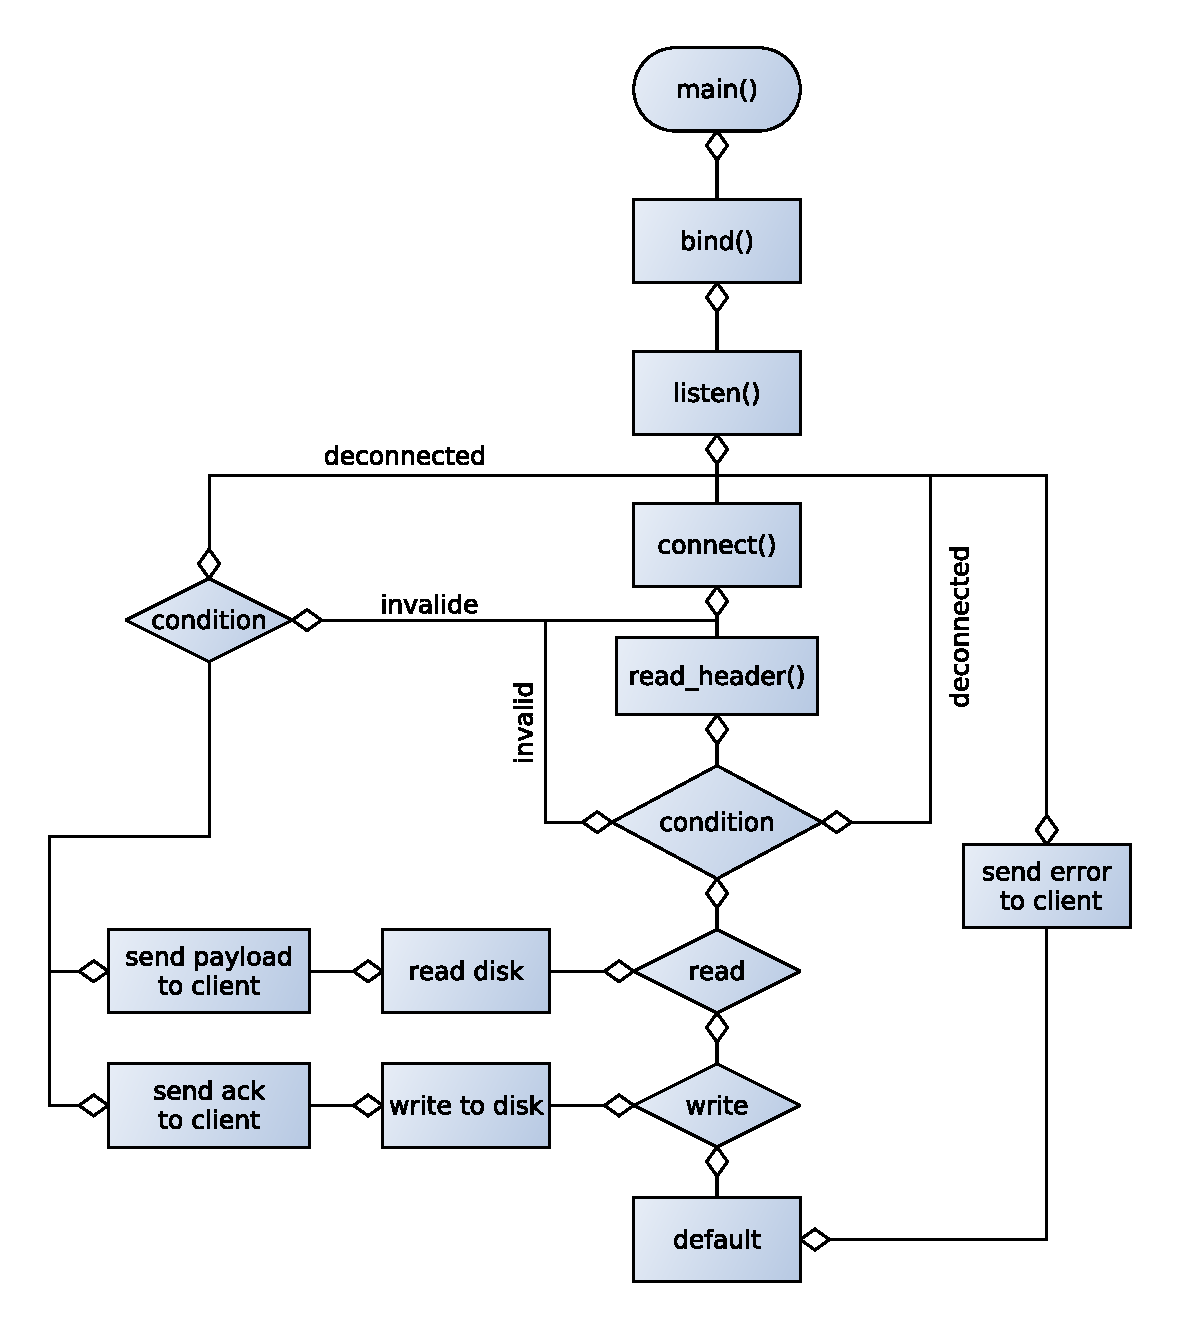
\includegraphics[scale=.6]{imgs/schema_server}
\caption{Principe de fonctionnement du server}
\label{fig:Architecture server}
\end{center}
\end{figure}

\subsection*{Solutions envisagées}

Une des solutions les plus simple serait de traiter les demandes l'une après l'autre; le client se connecte, envoie une requête, reçoit la réponse et se déconnecte. Le server fait la même chose; attend sur \emph{accept()} qu'un client se connecte puis traite la requête et y répond et se déconnecte.\\

Cette solution est simple, permet de mieux maîtriser l'état du client et du server mais est couteuse en connexions.\\


Une alternative possible est d'ajouter au protocole une requête (un message) de déconnexion qui synchronise le client et le server. Complexifier le protocole.\\

Une autre serait de faire une machine d'état afin de s'assurer de l'état dans lequel est le client et le server et le passage entre chaque état. Si un problème arrive, revenir dans un état connu.

\subsection*{Problème de client malicieux}

Si un client lance une requête et annonce une certaine longueur, le server va faire un read, tant que le client maintient la connexion et n'envoie pas les données, il bloque le server.\\

une solution serait de faire un \emph{select()} avant le read avec un timeout

\begin{lstlisting}[language=C, caption=pseudo code del\_entry()]
struct timeval tv;
fd_set readfds;
int state;

FD_ZERO(&readfds);

tv.tv_sec = 5;
tv.tv_usec = 0;

client = accept(s, (struct sockaddr *) &addr_client, (socklen_t *) &s_len);

FD_SET(client, &readfds);

boucle {

	state = select(n, &readfds, NULL, NULL, &tv);
	
	if(FD_ISSET(client, &readfds))
		read_socket();
	else
		continue;

...

}
\end{lstlisting}


\section{Exécution et tests unitaires}

Pour tester le fonctionnement\\


Où avec l'utilisation de strace

\begin{lstlisting}[language=bash,caption={lancer le server}]

	$ cp ./filesystems/minixfs\_lab1.img.org ./filesystems/minixfs\_lab1.img
	$ ./server 1234 ./filesystems/minixfs\_lab1.img
	
	$ strace ./server 1234 ./filesystems/minixfs\_lab1.img

	$ make run
	$ make run_debug
\end{lstlisting}

on peut enfin lancer le client\\
\begin{lstlisting}[language=bash,caption={lancer le client}]
	
	$ python2 tester_server.py
  
INFO:remote file system opened successfully
INFO:socket closed
INFO:remote file system opened successfully
(...)
.
----------------------------------------------------------------------
Ran 13 tests in 71.003s

OK

\end{lstlisting}


\section{Annexes}

\subsection*{ialloc()}

\begin{lstlisting}[language=C, caption=pseudo code ialloc()()]
ialloc(){

	recherche premier libre dans inode_map
	
	si not trouve:
		raise error plus aucun inode de libre
	
	inode trouve = occupe
	del ancien inode
	new inode
	
	return numero inode
}
\end{lstlisting}

\subsection*{ifree(inode)}

\begin{lstlisting}[language=C, caption=pseudo code ifree()()]
ifree( inode ){

	inode = libre
	return est-ce que inode est libre?
}
\end{lstlisting}

\subsection*{balloc()}

\begin{lstlisting}[language=C, caption=pseudo code balloc()()]
balloc( ){

	recherche premier block dans block map
	si non trouver:
		raise error plus de place sur disk
	
	block = occuper

	return numero de block
}
\end{lstlisting}

\subsection*{bfree(blocknum)}

\begin{lstlisting}[language=C, caption=pseudo code bfree()()]
bfree( data block ){

	data block = libre
	return est-ce que data block est libre?
}
\end{lstlisting}

\subsection*{bmap()}

\begin{lstlisting}[language=C, caption=pseudo code bmap()()]
bmap( numero inode, position relative block ){

	si block < 7:
		return position du nieme block direct
		
	block -= 7
	si block < nombre inode par block:
		return position du nieme block de indirect
	
	block -= nombre inode par block
	si block < (nombre inode par block)^2:
		adresse	data block = block / nombre inode par block
		position block = block mod nombre inode par block
		
		return numero block a adresse.posistion
		
	sinon:
		raise error depassement de capacite
}
\end{lstlisting}

\subsection*{add\_entry()}

\begin{lstlisting}[language=C, caption=pseudo code add\_entry()]
add_entry(inode dossier, nom fichier a inserer, inode du nouveau fichier){
	si nom de fichier non conforme;
		raise error
	si nom de fichier existe deja dans dossier:
		raise error
		
	tant que not done:
		prendre block dossier:
			si place libre:
				inserer inode et nom
				changer taille dossier
				done

			sinon:
				si not next block:
					creer nouveau block
					si plus possible creer:
						break
						
	si done:
		valider modification sur disk
	sinon:
		raise error plus de place
}
\end{lstlisting}


\end{document} 